\documentclass[10pt,twocolumn]{article}

\usepackage{graphicx}
\usepackage{amsmath,amssymb}
\usepackage{booktabs}
\usepackage{multirow}
\usepackage[hidelinks]{hyperref}
\usepackage{float}
\usepackage{placeins}
\usepackage{tabularx}
\usepackage{stfloats}
\raggedbottom

\title{Multimodal Fusion and Complementarity Analysis for Early Postoperative ICL Vault Prediction Using Preoperative AS-OCT and 2DAnalysis Measurements}
\author{Ding Yuan}
\date{}

\begin{document}

\maketitle

\begin{abstract}
Postoperative vault is a safety-relevant outcome after implantable collamer lens (ICL) implantation, but accurate preoperative prediction remains difficult. We evaluated whether preoperative AS-OCT images and CASIA2 2DAnalysis measurements contain complementary information for POD1 vault prediction, and whether this complementarity can be exploited by conventional or adaptive multimodal fusion under strict patient-level evaluation. Manually verified eye-level cohorts used POD1 vault only as the label and restricted inputs to preoperative data. Across five repeated patient-level splits, we evaluated modality-specific predictors, feature concatenation, leakage-safe validation-tuned additive late fusion, matched retrospective complementarity diagnostics, gate-based learnability diagnostics, and vault-range failure modes. In full-cohort repeated evaluation, measurement RF achieved MAE of $172.79 \pm 22.38~\mu$m, AS-OCT V0 achieved $173.78 \pm 15.77~\mu$m, and feature concatenation achieved $175.79 \pm 23.15~\mu$m. In the strict matched cohort, leakage-safe additive fusion achieved $171.94 \pm 20.22~\mu$m but did not show robust overall improvement over matched unimodal references. A retrospective Oracle Best-of-Two diagnostic achieved $132.45 \pm 26.11~\mu$m, indicating theoretical complementarity. Reliability-aware eye-specific gating achieved $171.84 \pm 28.64~\mu$m and likewise did not provide stable held-out improvement. High-Vault prediction and prediction-range compression remained persistent failure modes. These findings distinguish retrospective multimodal complementarity from its learnability and suggest that richer clinical, device, or surgical variables may be needed for extreme-vault prediction and weighting.
\end{abstract}

\section{Introduction}

Implantable collamer lens implantation is widely used to correct moderate-to-high myopia. Postoperative vault, the distance between the posterior ICL surface and the anterior crystalline lens surface, is central to postoperative safety. Excessively low vault may be associated with lens-contact and cataract risk, whereas excessively high vault may narrow the anterior chamber angle and elevate intraocular pressure~\cite{icl_sizing_rule,icl_vault_biometry}. A reliable preoperative estimate could therefore support lens selection, operative planning, and risk assessment~\cite{icl_vault_biometry,nakamura_icl_sizing}.

Preoperative vault prediction can draw on several forms of anterior-segment information. Structured biometric variables, including anterior chamber depth (ACD), white-to-white distance (WTW), crystalline lens rise (CLR), and angle-to-angle distance (ATA), provide compact and interpretable measurements that remain clinically useful~\cite{icl_sizing_rule,icl_vault_biometry,nakamura_icl_sizing,yang_vault_formula,wu_vault_formula}. Anterior segment optical coherence tomography (AS-OCT) provides cross-sectional imaging that may retain spatial morphology not fully captured by scalar measurements, while pretrained convolutional representations offer a practical way to use image information in modest clinical datasets~\cite{ophthalmic_deep_learning,as_oct_deep_learning,resnet,imagenet}. These two input families therefore provide distinct forms of preoperative information, without implying that their predictive errors are automatically complementary.

Multimodal modeling is attractive because feature concatenation, additive late fusion, or adaptive gating may combine information from imaging and structured measurements. However, the presence of distinct modality-specific information does not guarantee that a deployable fusion rule can improve prediction for unseen eyes. In particular, retrospective differences between unimodal errors must be distinguished from learnable complementarity: a fusion model must identify, using only inference-time information, when one modality should be trusted more than the other. This distinction is especially important in small clinical cohorts with fellow-eye structure, repeated partition sensitivity, and clinically important tail ranges.

This study asks whether preoperative AS-OCT images and CASIA2 2DAnalysis measurements contain complementary information for POD1 vault prediction, and whether this complementarity can be reliably exploited by conventional or adaptive multimodal fusion under strict patient-level evaluation. To address this question, we evaluate modality-specific predictors, conventional feature concatenation and leakage-safe validation-tuned additive late fusion, matched retrospective complementarity diagnostics, gate-based fusion learnability diagnostics, and failure modes across vault ranges and prediction range.

The contributions of this study are:
\begin{enumerate}
    \item We establish a patient-level multimodal evaluation of preoperative AS-OCT images and CASIA2 2DAnalysis measurements for POD1 vault prediction, separating modality-specific cohorts from strictly matched comparison cohorts.
    \item We systematically evaluate conventional multimodal fusion, including feature concatenation and leakage-safe validation-tuned additive late fusion, under repeated held-out patient-level splits.
    \item We quantify retrospective modality complementarity using matched prediction diagnostics and distinguish theoretical oracle headroom from deployable fusion performance.
    \item We assess whether observed complementarity can be translated into stable eye-specific weighting using gate-based learnability diagnostics, together with vault-range and prediction-range failure-mode analysis.
\end{enumerate}

\section{Related Work}

\subsection{Measurement-Based Vault Prediction}

Measurement-based methods estimate ICL size or postoperative vault from predefined anterior-segment variables. Established work has used WTW, ACD, ATA, CLR, and posterior-chamber or ciliary-sulcus descriptors in empirical rules, linear formulas, and machine-learning models~\cite{icl_vault_biometry,nakamura_icl_sizing,yang_vault_formula,wu_vault_formula}. These approaches are data-efficient and interpretable, which is valuable in modest clinical cohorts. Their limitation is representational: predefined measurements summarize selected axes and distances but cannot preserve the complete local spatial structure visible in the source scan. This motivates image-based quantitative prediction while retaining measurement models as strong clinical comparators.

\subsection{Image-Based Quantitative Prediction}

Medical image analysis spans segmentation or measurement extraction, end-to-end outcome regression, and transfer learning from pretrained visual encoders~\cite{medical_image_regression,ophthalmic_deep_learning}. Segmentation and extraction improve interpretability but depend on the selected anatomical targets. End-to-end regression can retain more spatial information but demands more data and is vulnerable to shortcut learning. Pretrained convolutional encoders provide an intermediate strategy: they retain image-level morphology while controlling the number of task-specific parameters. We therefore use an ImageNet-pretrained ResNet18 as a deliberately modest image baseline rather than claiming architectural novelty~\cite{resnet,imagenet}.

\subsection{Multimodal Representation and Fusion}

Multimodal fusion can occur at several levels~\cite{multimodal_learning_survey,huang_medical_fusion_review}. Early feature concatenation joins modality representations before prediction; late or additive fusion combines unimodal outputs; and dynamic gating assigns sample-specific weights. Tensor Fusion Networks explicitly model cross-modal products, while low-rank multimodal fusion factorizes these interactions to reduce computational cost~\cite{tfn,lmf}. Co-attention jointly conditions attention in two modalities, and cross-modal attention uses one modality to query another~\cite{coattention,mult}. These mechanisms differ from simple concatenation because they explicitly model interactions or conditional weighting.

The present work implements concatenation as a formal conventional multimodal baseline because it is transparent and capacity-controlled for the available cohort, and evaluates leakage-safe validation-tuned additive fusion as a conventional late-fusion baseline. Oracle best-of-two is used as a retrospective non-deployable diagnostic, and low-complexity gating is used for fusion learnability diagnostics. Tensor, co-attention, cross-modal attention, and Transformer fusion were not implemented and are not presented as study methods. General multimodal literature explains these mechanisms but does not establish their clinical effectiveness for ICL vault prediction.

\section{Methods}

\subsection{Study Overview}

This study evaluated preoperative prediction of POD1 ICL vault from two input sources: AS-OCT images and CASIA2 2DAnalysis measurements. Postoperative POD1 CASIA2 2DAnalysis reports were used only to define the eye-level vault label and were never used as predictive inputs. The analysis was organized into three layers: unimodal prediction, conventional multimodal fusion, and matched complementarity or fusion-learnability diagnostics.

An overview of the multimodal prediction and diagnostic framework is shown in Fig.~\ref{fig:multimodal_framework}.

\begin{figure*}[t]
\centering
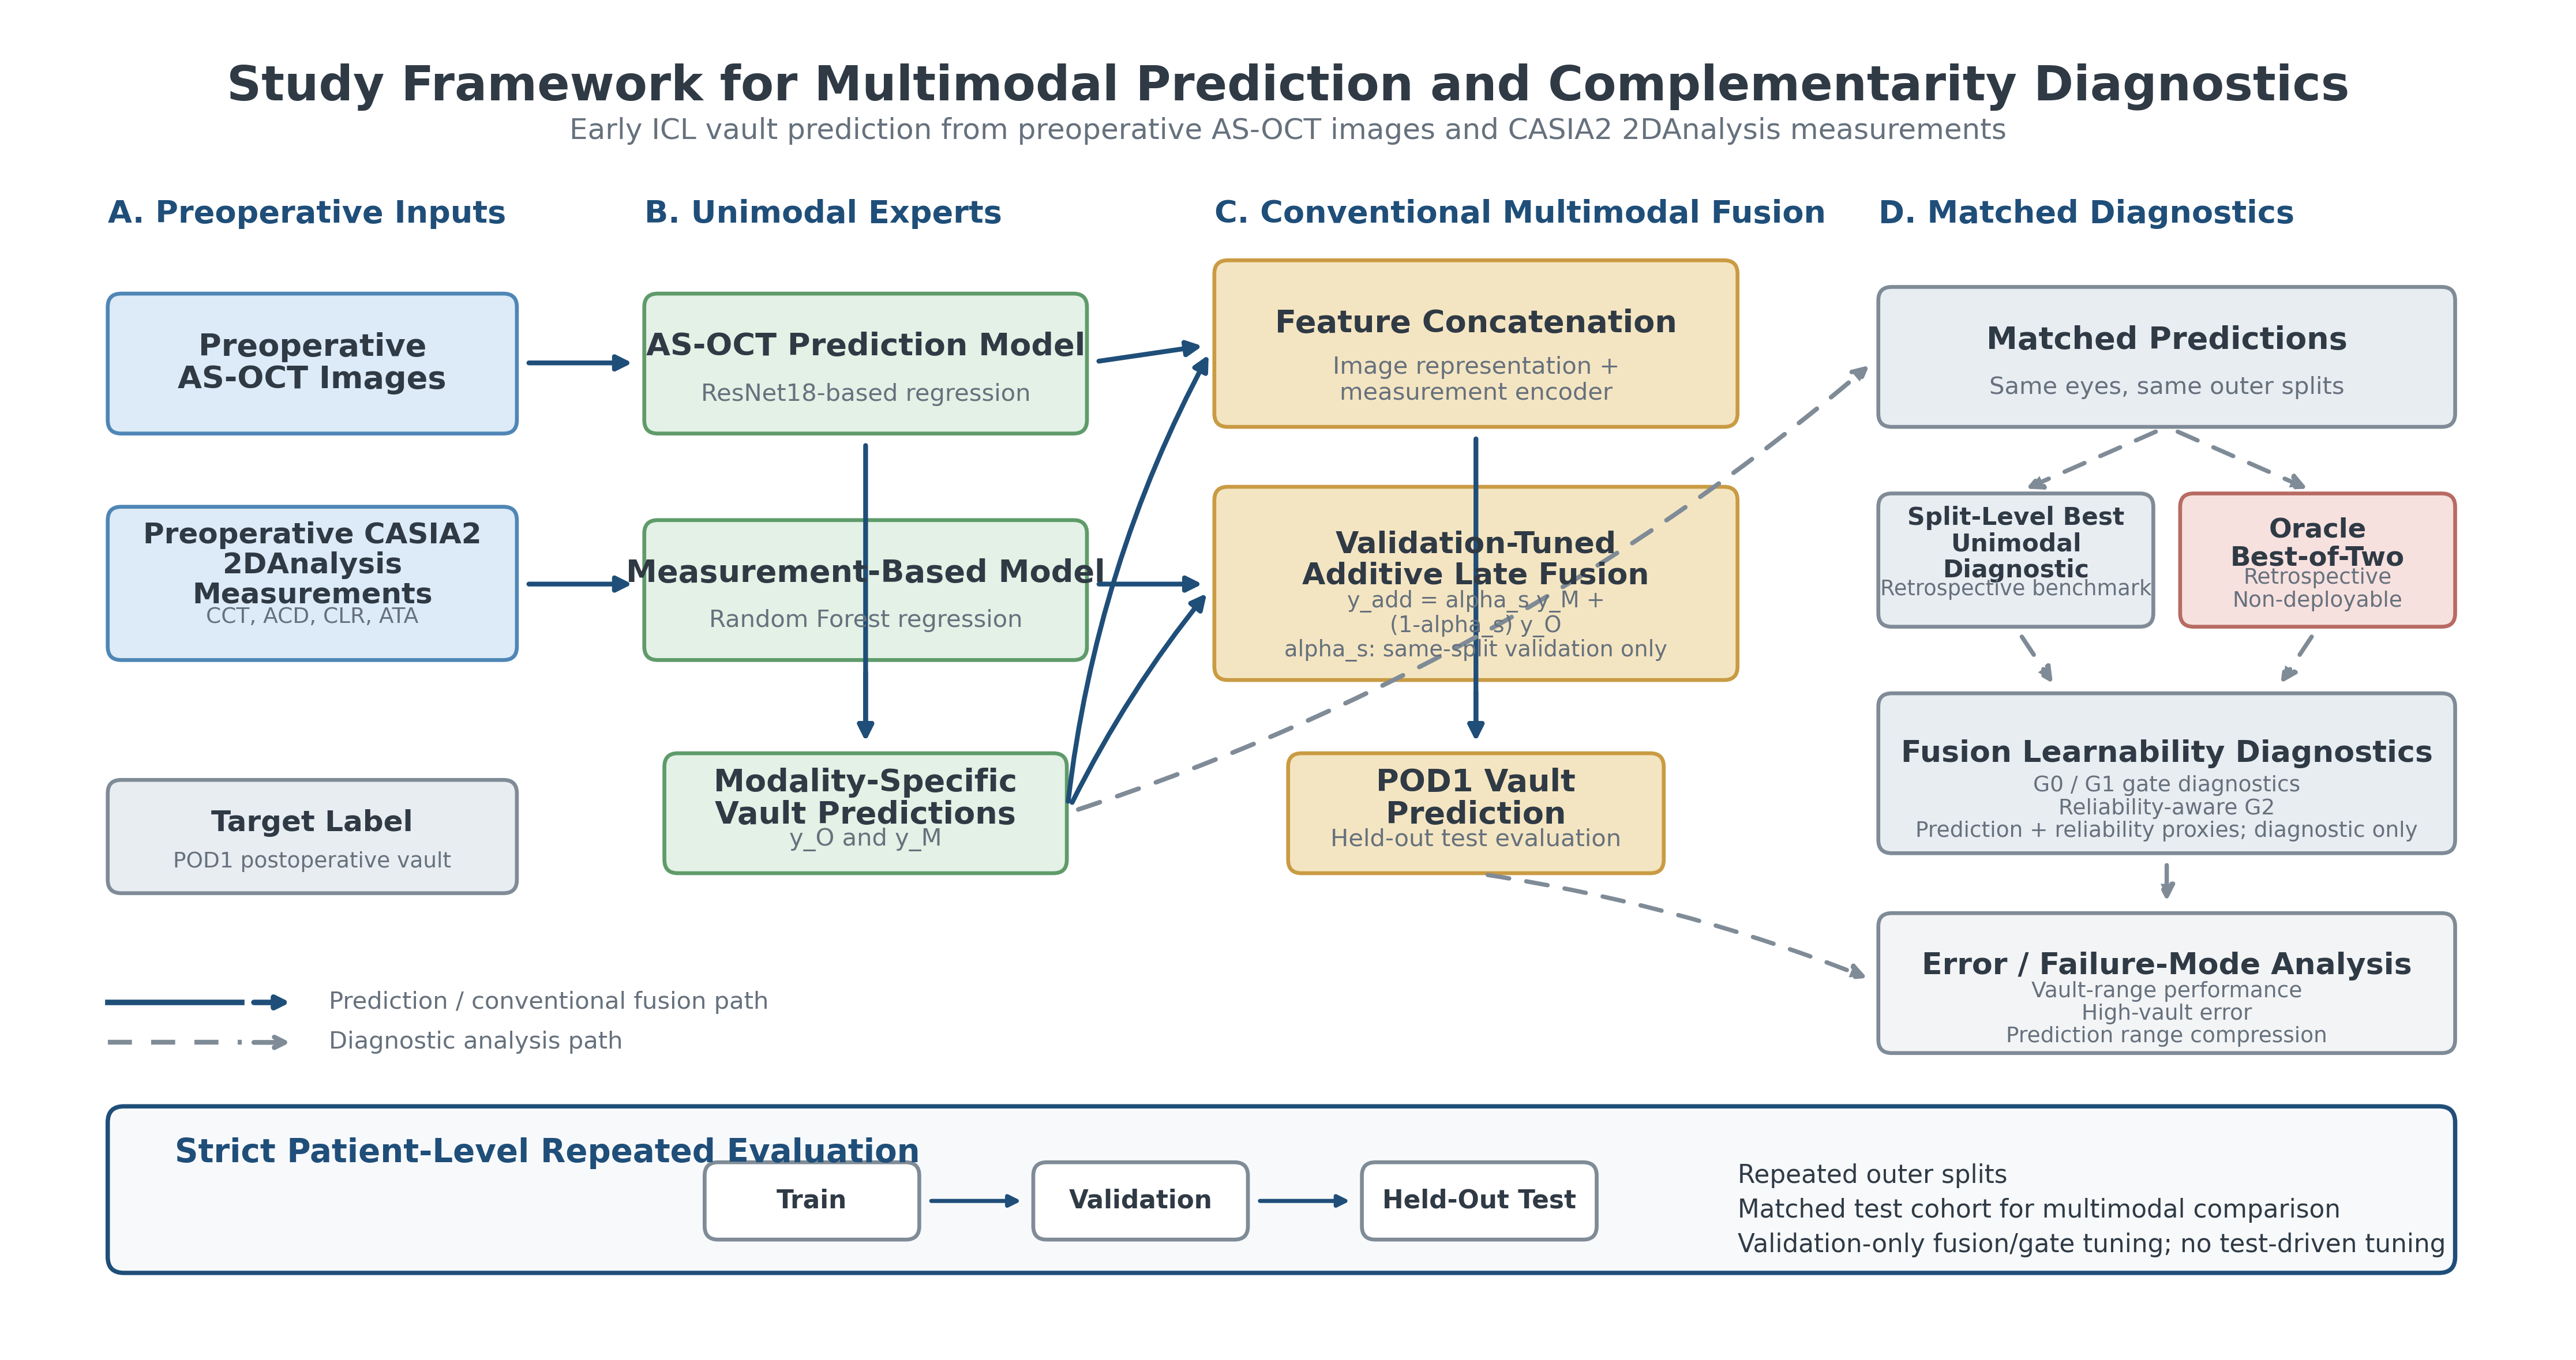
\includegraphics[width=0.98\textwidth]{figures/figure1_multimodal_framework_final.png}
\caption{Overview of the multimodal prediction and diagnostic framework. Preoperative AS-OCT images and CASIA2 2DAnalysis measurements were modeled using modality-specific predictors. Conventional multimodal fusion was evaluated using feature concatenation and leakage-safe validation-tuned additive late fusion. Matched predictions were further used to quantify retrospective modality complementarity and to assess the learnability of eye-specific modality weighting through gate-based diagnostics. All evaluations followed repeated patient-level splitting with validation-only model and fusion selection.}
\label{fig:multimodal_framework}
\end{figure*}

Two evaluation populations were distinguished throughout the protocol. Modality-specific full cohorts were used to characterize the frozen AS-OCT, measurement, and concat-fusion baselines according to their actual input availability. A stricter matched cohort was then used for fair comparison of unimodal predictions, additive fusion, oracle complementarity, and gate diagnostics on identical eyes and split assignments. The matched analyses were therefore designed to separate true same-eye modality interaction from differences in cohort composition.

For eye $i$, let $x_i^{O}$ denote the preoperative AS-OCT input, $x_i^{M}$ the structured preoperative measurement vector, and $y_i$ the verified POD1 vault in micrometers. The unimodal predictors are denoted as $\hat{y}_i^{O}$ for AS-OCT and $\hat{y}_i^{M}$ for measurements. Multimodal analyses evaluate whether these predictors or their learned representations can be combined under patient-level train, validation, and test separation.

\subsection{AS-OCT Prediction Model}

The frozen AS-OCT baseline used a selected preoperative AS-OCT image as input. Images were resized to $224 \times 224$ pixels and passed through an ImageNet-pretrained ResNet18 encoder~\cite{resnet,imagenet}. The classification layer was replaced by a scalar regression head:
\begin{equation}
z_i^{O}=E_{O}(x_i^{O}), \qquad
\hat{y}_i^{O}=R_{O}(z_i^{O}).
\end{equation}
The model was trained with MSE loss on train-normalized vault labels, batch size 16, learning rate $10^{-4}$, weight decay $10^{-4}$, and validation-based checkpoint selection by MAE. The backbone was fine-tuned rather than frozen. Primary AS-OCT evaluation used a three-seed ensemble, whereas repeated-split evaluation used the frozen single-seed protocol across the predefined outer splits. Transformer, Mamba, ROI-cropping, multi-view pooling, and range-aware AS-OCT variants were exploratory or screening analyses and were not part of the main Method.

\subsection{Measurement-Based Prediction Model}

The measurement model used five verified preoperative CASIA2 2DAnalysis variables:
\begin{equation}
x_i^{M}=[\mathrm{CCT},\mathrm{ACD}_{epi},\mathrm{ACD}_{endo},
\mathrm{CLR},\mathrm{ATA}]_i .
\end{equation}
CCT and CLR followed the frozen micrometer convention; ACD Epi, ACD Endo, and ATA were represented in millimeters. The measurement-only manifests required complete numeric values for all five inputs, so no measurement imputation was used in the formal baseline. Candidate linear regression, ridge regression, MLP, and RF models were evaluated on the validation partition in the frozen baseline study. The formal measurement baseline was an RF regressor with 500 trees, minimum leaf size 2, and random state 42, trained on the training partition and evaluated after model selection on the validation partition.

\subsection{Conventional Multimodal Fusion}

\subsubsection{Feature Concatenation}

Feature concatenation was implemented as a conventional multimodal baseline rather than a novel fusion architecture. The image branch used the same ImageNet-pretrained ResNet18 representation as the AS-OCT model. The five preoperative measurement variables were standardized using training-split statistics and projected through a small MLP measurement encoder. The image representation and measurement representation were concatenated and passed to an MLP regression head:
\begin{equation}
z_i^{F}=[z_i^{O};E_M(x_i^{M})], \qquad
\hat{y}_i^{F}=R_F(z_i^{F}).
\end{equation}
The concat model used label-normalized MSE, batch size 16, learning rate $10^{-4}$, weight decay $10^{-4}$, and validation-based checkpoint selection. This baseline did not implement cross-attention, Transformer interaction, tensor fusion, or dynamic modality selection.

\subsubsection{Leakage-Safe Validation-Tuned Additive Fusion}

Additive fusion was evaluated as conventional prediction-level late fusion of the frozen unimodal predictors. For outer split $s$ and test eye $i$, the fused prediction was
\begin{equation}
\hat{y}_{i,s}^{add}
=
\alpha_s \hat{y}_{i,s}^{M}
+
(1-\alpha_s)\hat{y}_{i,s}^{O},
\end{equation}
where $\alpha_s$ is the Measurement weight and $1-\alpha_s$ is the AS-OCT weight.

For each outer split, $\alpha_s$ was selected exclusively from that split's validation partition:
\begin{equation}
\alpha_s =
\arg\min_{\alpha \in \{0,0.05,\ldots,1\}}
\mathrm{MAE}_{val,s}(\alpha).
\end{equation}
The selection metric was validation MAE. When multiple grid values were within $0.5~\mu$m of the best validation MAE, the largest $\alpha$ was selected according to the frozen tie rule. Each selected $\alpha_s$ was then frozen and applied only to the corresponding held-out test partition. No pooled cross-split validation objective and no test-label tuning were used.

\subsection{Matched Modality Complementarity Analysis}

Matched analyses used Measurement RF and AS-OCT V0 predictions generated on the same fusion-cohort split assignments. Predictions were aligned by split seed, sample identifier, patient identifier, eye, and ground-truth vault before computing any interaction diagnostic. This matched protocol was used for comparison of unimodal predictors, concat fusion, additive fusion, and diagnostic complementarity measures.

The matched best unimodal benchmark was defined separately for each outer split as the lower-MAE unimodal predictor between Measurement RF and AS-OCT V0 at split level. It is a retrospective split-level diagnostic benchmark and not a deployable prospectively selected model.

Oracle Best-of-Two was defined for each matched test eye by choosing the smaller absolute error between the two unimodal predictions:
\begin{equation}
e_i^{oracle}
=
\min \left(
|\hat{y}_i^{M}-y_i|,
|\hat{y}_i^{O}-y_i|
\right).
\end{equation}
The oracle uses test labels post hoc to quantify theoretical modality complementarity. It was never used for model fitting or model selection, is not deployable, and is not a fusion algorithm.

\subsection{Fusion Learnability Diagnostics}

Fusion learnability diagnostics tested whether retrospective modality complementarity could be converted into a prospective eye-specific weighting rule using only information available at inference time. G0 and G1 were validation-only diagnostics based on patient-grouped nested cross-validation within each outer validation split. G0 used prediction-derived features, while G1 additionally considered the five preoperative measurements. These diagnostics were used to decide whether the available signals justified formal adaptive fusion evaluation.

Reliability-aware G2 was a linear soft gate fit separately within each outer split. For eye $i$, the gate used
\begin{equation}
\alpha_i=\sigma(w^T z_i+b),
\end{equation}
\begin{equation}
\hat{y}_i^{G2}
=
\alpha_i \hat{y}_i^{O}
+
(1-\alpha_i)\hat{y}_i^{M}.
\end{equation}
In G2, $\alpha_i$ is the AS-OCT weight. This alpha is distinct from the additive-fusion $\alpha_s$, which is the Measurement weight.

The G2 input vector was
\begin{equation}
z_i=[
\hat{y}_i^{O},
\hat{y}_i^{M},
|\hat{y}_i^{O}-\hat{y}_i^{M}|,
d_i^{O},
q_i^{O},
d_i^{M}
],
\end{equation}
where $d_i^{O}$ is the AS-OCT view-wise prediction dispersion after imputation, $q_i^{O}$ is a single-view indicator, and $d_i^{M}$ is the RF tree prediction dispersion. These quantities were treated as prediction-dispersion reliability proxies, not as calibrated uncertainty estimates.

For AS-OCT eyes with at least two preoperative views, raw view dispersion was the population standard deviation of view-wise predictions from the frozen matched AS-OCT V0 checkpoint for that outer split. For eyes with a single view, raw view dispersion was undefined. Within each outer split, the imputation value was the median raw dispersion among multi-view eyes in that split's validation partition. The same validation-derived value was applied to validation and test single-view eyes, together with the explicit single-view indicator. Test feature distributions and test labels were not used to compute the imputation value.

Measurement reliability was summarized by the population standard deviation of predictions across the 500 RF trees. G2 feature scaling, gate fitting, and single-view imputation were performed using the validation partition only. The gate was optimized on validation rows with full-batch gradient descent, Smooth-L1 loss with $\beta=25~\mu$m on the fused vault prediction, learning rate 0.03, L2 penalty $10^{-4}$, and 2500 iterations. After these quantities were frozen, the gate was evaluated once on the corresponding held-out test partition.

\subsection{Evaluation Protocol}

All data splits were assigned at patient level so that eyes from the same patient could not appear across train, validation, and test partitions within a split. The formal repeated outer split seeds were 42, 1001, 2002, 2026, and 3407. For each outer split, model fitting used the training partition, model or weight selection used the validation partition, and final evaluation used the held-out test partition.

For conventional additive fusion, the fusion weight was selected only from the same split's validation predictions and labels before held-out test evaluation. For G2, the scaler, gate coefficients, RF-tree dispersion model, AS-OCT view-dispersion imputation value, and all other gate-training quantities were fitted or estimated within the same split without test-label tuning. All matched multimodal comparisons used the same matched test assignments for Measurement RF, AS-OCT V0, concat fusion, additive fusion, G2, matched best unimodal, and Oracle Best-of-Two.

MAE was the primary evaluation metric. RMSE and $R^2$ were secondary global metrics. Vault strata were defined as low ($<250~\mu$m), medium (250--750~$\mu$m), and high ($>750~\mu$m). Range-specific analyses reported stratum-specific MAE and signed error. Prediction-range compression was summarized by the ratio of the prediction range to the observed target range, with the prediction standard deviation to target standard deviation ratio used as a related dispersion summary.

\section{Experiments and Results}

\subsection{Cohort and Evaluation Cohorts}

Table~\ref{tab:v5_cohort} summarizes the frozen full-cohort v5 datasets used for modality-specific baseline characterization. These cohorts reflect actual input availability for AS-OCT, measurement, and concat-fusion experiments. All labels and required features were complete in their corresponding manifests, all AS-OCT paths required by image settings were present, and split QC found no patient leakage or duplicate samples.

\begin{table}[t]
\centering
\caption{Frozen v5 cohort composition.}
\label{tab:v5_cohort}
\footnotesize
\setlength{\tabcolsep}{3pt}
\begin{tabular}{lrrrrr}
\toprule
Setting & Eyes & Patients & Low & Medium & High \\
\midrule
AS-OCT-only & 392 & 208 & 11 & 289 & 92 \\
Measurement-only & 373 & 201 & 11 & 273 & 89 \\
Fusion & 372 & 201 & 11 & 272 & 89 \\
\bottomrule
\end{tabular}
\end{table}

For the primary split, AS-OCT contained 274/59/59 train/validation/test eyes, measurement-only contained 261/56/56, and fusion contained 260/56/56. The corresponding patient counts were 146/31/31 for AS-OCT and 141/30/30 for measurement and fusion. Strict matched v5.2 analyses were performed separately on the common fusion-cohort split assignments, yielding 280 repeated held-out test predictions across five outer splits. Matched analyses were used for fair comparison of Measurement RF, AS-OCT V0, concat fusion, leakage-safe additive fusion, G2, matched best unimodal, and Oracle Best-of-Two.

\subsection{Unimodal Prediction Performance}

Table~\ref{tab:v5_main_results} reports the frozen full-cohort primary and repeated results. On the primary split, the AS-OCT three-seed ensemble achieved the lowest MAE of 175.00~$\mu$m, compared with 200.79~$\mu$m for measurement RF and 193.50~$\mu$m for concat fusion. Across five repeated patient-level splits, measurement RF achieved the lowest mean MAE at $172.79 \pm 22.38~\mu$m, while AS-OCT was close at $173.78 \pm 15.77~\mu$m. Thus, the full-cohort results support two competitive unimodal predictors rather than a uniformly dominant modality.

\begin{table*}[t]
\centering
\caption{Frozen v5 primary and repeated patient-level results.}
\label{tab:v5_main_results}
\footnotesize
\setlength{\tabcolsep}{5pt}
\begin{tabular}{lrrrrr}
\toprule
Model & Primary MAE & Primary RMSE & Primary $R^2$ & Primary range ratio & Repeated MAE \\
\midrule
Measurement-only RF & 200.79 & 247.53 & 0.194 & 0.539 & $172.79 \pm 22.38$ \\
AS-OCT 3-seed ensemble & 175.00 & 217.19 & -0.011 & 0.459 & $173.78 \pm 15.77$ \\
Concat fusion 3-seed ensemble & 193.50 & 254.60 & 0.148 & 0.305 & $175.79 \pm 23.15$ \\
\bottomrule
\end{tabular}
\end{table*}

\subsection{Conventional Multimodal Fusion Performance}

Simple feature concatenation did not improve over the unimodal baselines in the full-cohort repeated evaluation, with repeated MAE of $175.79 \pm 23.15~\mu$m. In the strict matched cohort, concat fusion also failed to exceed the retrospectively identified matched best unimodal predictor in any outer split.

Leakage-safe validation-tuned additive fusion was then evaluated on the same matched outer splits using only each split's validation partition to select the Measurement weight before held-out test evaluation. This protocol produced repeated MAE of $171.94 \pm 20.22~\mu$m, won 3/5 splits against the matched best unimodal diagnostic, and won 4/5 splits against concat fusion. The selected Measurement weights varied substantially across splits (0.05--0.90), and the result did not demonstrate a robust overall improvement over matched unimodal references.

Table~\ref{tab:v52_matched} summarizes the matched repeated-split comparison. Matched best unimodal is a retrospective split-level diagnostic benchmark, not a deployable model. Oracle Best-of-Two is a retrospective per-eye diagnostic lower bound, not a fusion algorithm.

\begin{table*}[t]
\centering
\caption{Strict matched v5.2 repeated-split multimodal comparison. Deployable predictors and retrospective diagnostics are shown together to separate held-out prediction performance from non-deployable complementarity estimates.}
\label{tab:v52_matched}
\footnotesize
\setlength{\tabcolsep}{4pt}
\begin{tabular}{llcc}
\toprule
Method & Role & Repeated MAE & Wins vs matched best \\
\midrule
Measurement RF & Deployable unimodal baseline & $172.08 \pm 23.35$ & 0/5 \\
AS-OCT V0 & Deployable unimodal baseline & $179.98 \pm 25.58$ & 0/5 \\
Concat fusion & Deployable conventional fusion & $175.79 \pm 23.15$ & 0/5 \\
Leakage-safe additive fusion & Deployable conventional late fusion & $171.94 \pm 20.22$ & 3/5 \\
Matched best unimodal & Retrospective split-level diagnostic & $170.02 \pm 23.53$ & Reference \\
Oracle Best-of-Two & Retrospective per-eye diagnostic & $132.45 \pm 26.11$ & Diagnostic \\
G2 reliability-aware gate & Diagnostic adaptive gate & $171.84 \pm 28.64$ & 1/5 \\
\bottomrule
\end{tabular}
\end{table*}

The five full-cohort repeated-split test MAEs were 200.79, 171.03, 175.54, 178.15, and 138.43~$\mu$m for measurement RF; 181.55, 168.90, 161.55, 159.52, and 197.39~$\mu$m for AS-OCT; and 203.29, 163.41, 174.79, 192.52, and 144.92~$\mu$m for concat fusion. The ranking changed across partitions, reinforcing the need for repeated patient-level evaluation rather than a single favorable split.


\begin{figure*}[t]
\centering
\includegraphics[width=0.95\textwidth]{figures/fig_v5_overall_comparison.pdf}
\caption{Frozen v5 comparison. (a) Test MAE across five repeated patient-level splits. (b) Range-specific MAE for low-, medium-, and high-vault eyes. (c) Prediction-range ratio, where lower values indicate stronger compression.}
\label{fig:v5_overall}
\end{figure*}

\subsection{Vault-Range and Prediction-Range Behavior}

Table~\ref{tab:v5_range} reports matched repeated-split range behavior using the low ($<250~\mu$m), medium (250--750~$\mu$m), and high ($>750~\mu$m) vault strata. Medium-vault eyes dominated the cohorts and had substantially lower error than the high-vault group. The low-vault test subsets were very small, so low-vault means are unstable and should not be used for strong model ranking. High-vault MAE remained large for all deployable and diagnostic fusion methods. Leakage-safe additive fusion had High-Vault MAE of 345.28~$\mu$m, and G2 had High-Vault MAE of 351.98~$\mu$m; neither resolved the high-vault failure mode.

\begin{table}[t]
\centering
\caption{Matched repeated-split range-specific MAE and prediction-range compression.}
\label{tab:v5_range}
\footnotesize
\setlength{\tabcolsep}{2pt}
\resizebox{\columnwidth}{!}{%
\begin{tabular}{lrrrr}
\toprule
Model & Low MAE & Medium MAE & High MAE & Range ratio \\
\midrule
Measurement RF & 341.21 & 129.56 & 309.27 & 0.505 \\
AS-OCT V0 & 297.19 & 122.76 & 369.05 & 0.367 \\
Concat fusion & 255.62 & 127.08 & 333.16 & 0.402 \\
Leakage-safe additive & 315.47 & 122.07 & 345.28 & 0.387 \\
G2 reliability-aware gate & 295.61 & 117.72 & 351.98 & 0.402 \\
\bottomrule
\end{tabular}
}
\end{table}

All matched predictors showed prediction-range compression, with range ratios substantially below one. The leakage-safe additive range ratio was 0.387, similar to AS-OCT and concat and lower than measurement RF. Additive averaging therefore did not correct the dynamic-range compression that contributes to tail errors.

\subsection{Matched Modality Complementarity}

The strict matched audit covered all 280/280 repeated test predictions. Oracle Best-of-Two achieved repeated MAE of $132.45 \pm 26.11~\mu$m, compared with $170.02 \pm 23.53~\mu$m for the matched best unimodal diagnostic, leaving 37.57~$\mu$m of retrospective per-eye headroom. In the high-vault stratum, Oracle Best-of-Two achieved MAE of 277.72~$\mu$m, lower than the deployable unimodal and fusion methods.

This oracle result shows that the two modalities contain retrospective individual-eye complementarity. It does not imply that oracle performance is achievable prospectively, because the oracle uses the test label to choose the smaller absolute error for each eye. Leakage-safe additive fusion had mean oracle fraction captured of -0.050, indicating that this simple validation-tuned late fusion did not capture positive oracle headroom on average.

\subsection{Fusion Learnability Diagnostics}

G0 and G1 tested whether the better unimodal predictor could be identified prospectively from inference-time signals. G0 prediction-only features produced winner AUC of $0.521 \pm 0.069$, OOF MAE of $163.88 \pm 22.46~\mu$m, won 2/5 splits against nested fixed alpha, and captured a negative fraction of oracle headroom (-0.0928). G1 prediction-plus-measurement features produced winner AUC of $0.456 \pm 0.107$, OOF MAE of $165.77 \pm 21.20~\mu$m, won 1/5 splits, and also captured negative oracle headroom (-0.1599). Both diagnostics therefore met the predefined NO-GO interpretation.

The formal corrected G2 reliability-aware gate was evaluated as a diagnostic adaptive fusion experiment, not as the proposed final predictor. It achieved repeated MAE of $171.84 \pm 28.64~\mu$m, won 1/5 splits against the matched best unimodal diagnostic, and had High-Vault MAE of 351.98~$\mu$m. Its mean near-extreme alpha fraction was 0.825, and gate coefficients showed mixed signs across splits. Under the leakage-safe correction, additive fusion beat G2 in 3/5 splits, but the central result is not that one fusion variant is definitively superior. Rather, neither leakage-safe additive fusion nor reliability-aware eye-specific gating consistently translated retrospective oracle complementarity into improved held-out prediction.

\subsection{Summary of Main Findings}

The repeated full-cohort baselines showed competitive Measurement RF and AS-OCT unimodal predictors, while simple concat fusion did not provide stable benefit. In the strict matched cohort, leakage-safe validation-tuned additive fusion was a modest conventional baseline with split-dependent gains but no robust overall improvement over matched unimodal references. Oracle Best-of-Two demonstrated substantial retrospective per-eye complementarity, yet G0/G1/G2 diagnostics did not show that the available inference-time signals could reliably learn which modality to trust. High-vault error and prediction-range compression remained unresolved.

\section{Discussion}

\subsection{Principal Findings}

This study found that both preoperative AS-OCT images and CASIA2 2DAnalysis measurements contain predictive signal for POD1 vault, but neither conventional nor adaptive fusion converted that signal into robust held-out improvement. The leakage-safe additive fusion result was competitive at $171.94 \pm 20.22~\mu$m, but did not establish stable superiority over matched unimodal references. In contrast, the retrospective Oracle Best-of-Two showed 37.57~$\mu$m of headroom, indicating that the modalities made partially non-overlapping errors on the same test eyes. The central finding is therefore that retrospective modality complementarity does not imply learnable complementarity under the current inputs, cohort size, and reliability proxies.

\subsection{Retrospective Multimodal Complementarity}

The matched analysis was essential because the full AS-OCT, measurement, and concat cohorts differed in input availability. Once predictions were aligned on identical held-out eyes and split assignments, the large gap between individual unimodal predictors and the retrospective Oracle Best-of-Two suggested that AS-OCT and measurement predictions do not fail on exactly the same eyes. This supports retrospective predictive complementarity: each modality sometimes contains information or error structure not captured by the other.

This interpretation must remain limited. Oracle Best-of-Two uses the test label post hoc to choose the smaller absolute error, so it measures theoretical headroom rather than a deployable decision rule. It should not be interpreted as biological complementarity by itself, nor as evidence that a new eye can be assigned to the better modality before the outcome is known. The practical problem is not only whether the modalities differ, but whether the available preoperative signals reveal when each modality should be trusted.

\subsection{Why Fusion Did Not Reliably Exploit Complementarity}

Feature concatenation provides a direct and transparent multimodal baseline, but it does not explicitly solve the trust-assignment problem. In this cohort, image representations and tabular measurements may have been difficult to align, partly redundant, or insufficiently informative about modality reliability. These are possible explanations rather than proven mechanisms. The observed result only supports the narrower conclusion that simple concatenation did not consistently improve prediction under the frozen protocol.

Leakage-safe additive fusion was more competitive than concat in most outer splits, winning 4/5 splits against concat and 3/5 against the matched best unimodal diagnostic. However, its repeated MAE did not show robust overall superiority over the matched unimodal references. It should therefore be interpreted as a simple conventional late-fusion baseline with split-dependent gains, not as a stable positive fusion result. The validation-selected Measurement weights also varied substantially across outer splits (0.90, 0.55, 0.05, 0.40, and 0.05), suggesting that a single stable population-level modality balance was difficult to identify in the current cohort. Because these weights were split-level quantities, they should not be interpreted as evidence that different individual patients require different fixed modality weights.

\subsection{Fusion Learnability Diagnostics}

The oracle result naturally motivates a second question: whether the better modality can be identified at inference time. G0, G1, and G2 were designed as diagnostics for this question, not as evidence that a more complex fusion architecture should be adopted. G0 and G1 showed near-chance or below-chance winner discrimination, and the formal corrected G2 gate achieved $171.84 \pm 28.64~\mu$m with only 1/5 wins against the matched best unimodal diagnostic. The predefined interpretation therefore remained NO-GO for adaptive reliability-aware fusion.

The gate diagnostics help explain why oracle headroom was not prospectively captured. Near-extreme G2 weights were frequent, and coefficient directions changed across splits. These patterns are consistent with a model that is difficult to estimate robustly from the available validation data, but they should not be overstated as proof of a specific overfitting mechanism. The stronger conclusion is methodological: observing partially non-overlapping modality errors is not enough. A deployable gate also requires reliable inference-time features that indicate which modality is more trustworthy for a new eye.

\subsection{Persistent High-Vault Error and Prediction Range Compression}

High-vault prediction remained the main clinically relevant failure mode. In the matched analysis, leakage-safe additive fusion and G2 had High-Vault MAEs of 345.28~$\mu$m and 351.98~$\mu$m, respectively, while the Oracle Best-of-Two remained lower at 277.72~$\mu$m. This pattern again separates retrospective headroom from learnable improvement: the two unimodal predictors sometimes contain useful tail information, but the evaluated fusion strategies did not reliably recover it.

Prediction-range compression provides one plausible explanation for persistent errors at the tails. The model predictions occupied a narrower dynamic range than the observed vault labels, and the leakage-safe additive range ratio was 0.387. Such compression is compatible with regression-to-the-mean behavior in a modest and imbalanced cohort, where medium-vault eyes dominate the objective and extreme vaults are sparse. However, the present analysis does not prove that compression arises from any single network architecture or loss function. Future studies should continue to report both global MAE and range-specific behavior, because average-error gains can obscure clinically important tail failures.

\subsection{Methodological Implications and Limitations}

The main contribution of this work is not a new fusion architecture. It lies in a leakage-controlled, patient-level, matched evaluation that separates three questions often conflated in multimodal medical prediction: whether each modality predicts the outcome, whether their errors are retrospectively complementary, and whether that complementarity is learnable for held-out deployment. The combination of matched Oracle analysis and gate learnability diagnostics provides a disciplined way to distinguish ``complementarity exists'' from ``complementarity can be used by a deployable fusion model.''

Several limitations remain. The study is retrospective, single-project, and modest in size, with no external validation. Repeated splits reduce dependence on one partition but do not replace independent validation, and repeated-test pooled eye-level diagnostics may contain the same physical eye in multiple outer test splits. Low- and high-vault eyes are relatively sparse, limiting tail-specific inference. The formal predictors used only two preoperative modality families: AS-OCT images and five CASIA2 2DAnalysis measurements. Device- and procedure-related variables such as ICL size, model, power, orientation, and other surgical factors were not available as formal inputs and may contain information needed for reliable fusion or extreme-vault prediction. Future studies should assess whether incorporating such variables improves modality trust estimation and tail performance. Finally, the reliability features used in G2 were prediction-dispersion proxies rather than calibrated uncertainty estimates, and the NO-GO result applies to the evaluated strategies, current inputs, and current cohort rather than to every possible multimodal model.

\section{Conclusion}

This study systematically evaluated POD1 ICL vault prediction from preoperative AS-OCT images and CASIA2 2DAnalysis measurements under repeated patient-level splitting, conventional fusion, matched complementarity analysis, and adaptive fusion diagnostics. The findings indicate that the two modalities contain retrospective complementary predictive information, but the evaluated feature-concatenation, leakage-safe additive late-fusion, and gate-based adaptive strategies did not consistently translate this complementarity into improved held-out prediction under the current cohort and input setting. High-Vault error and prediction-range compression remained persistent limitations. Future work should assess whether richer clinical, device, and surgical variables can improve extreme-vault prediction and provide more informative signals for multimodal fusion.

\begingroup
\small
\bibliographystyle{IEEEtran}
\bibliography{references}
\endgroup

\end{document}
